\section{Introduction}

This report was conceived about the study of a Recycling Folded Cascode (RFC) Operational Transconductance Amplifier (OTA) circuit\textsuperscript{\cite{artigo-prof}}. The main goal of this study was to design and simulate the circuit, and observing the advantages of RFC OTA over the conventional Folded Cascode (FC) OTA. 

The circuit was designed using the TSMC 65nm technology and the design was done using the Cadence Virtuoso software. In Figure \ref{fig:OTA_schematic} is the proposed circuit schematic.

\begin{figure}[H]
    \centering
    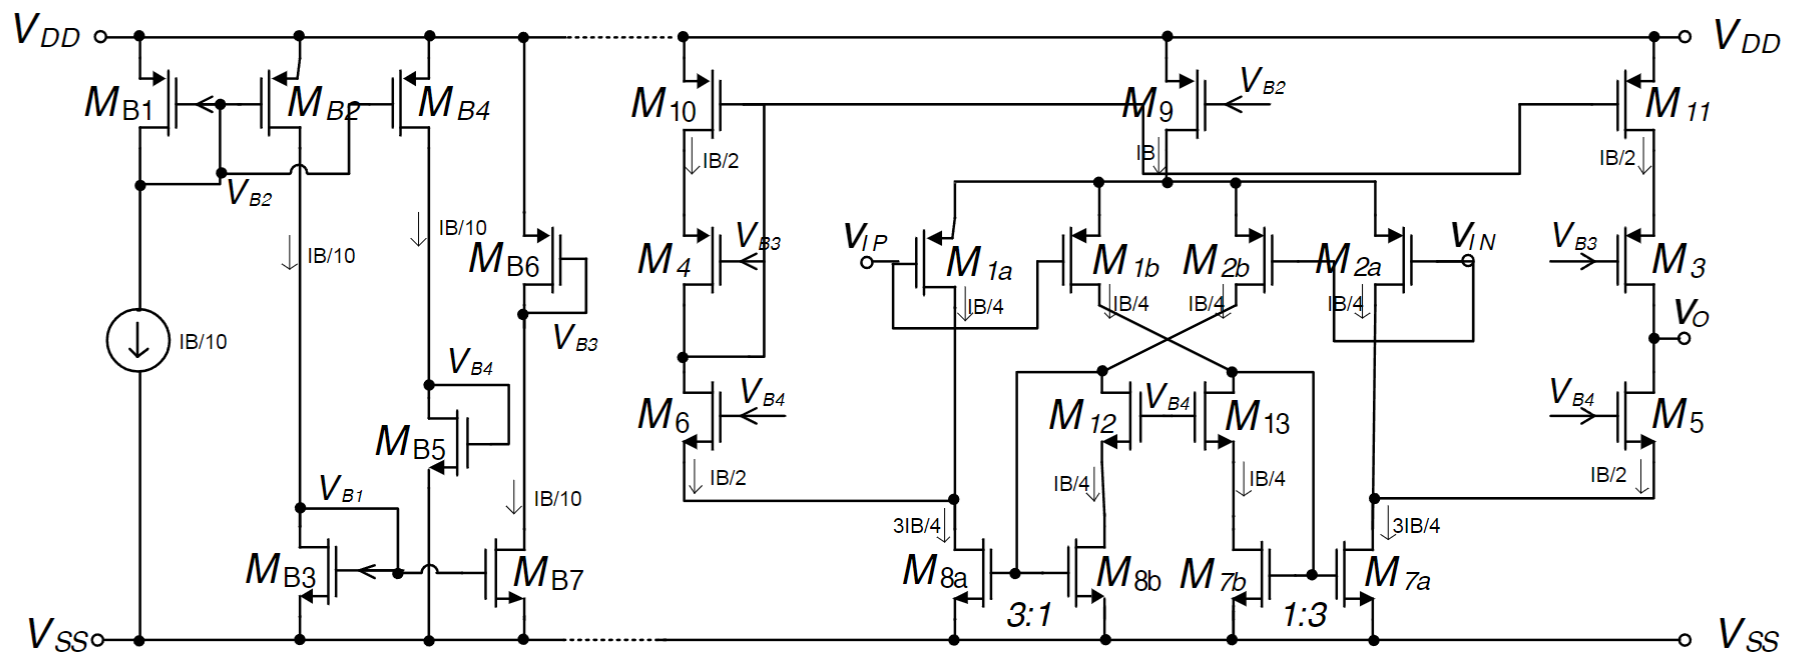
\includegraphics[width=1\textwidth]{Images/RFC_OTA_schematic.png}
    \caption{Recycling Folded Cascode OTA Schematic\textsuperscript{\cite{Lab-statement}}}
    \label{fig:OTA_schematic}
\end{figure}

\begin{table}[h]
    \centering
    \caption{Goals and Constraints}
    \begin{tabularx}{\textwidth}{>{\centering\arraybackslash}X >{\centering\arraybackslash}X}
        \toprule
        \textbf{Goal/Constraint} & \textbf{Description}\\
        \midrule
        DC Gain & $A_{min}\geq 66dB$\\
        \midrule
        Gain Bandwidth Product ($C_L = 2pF$) & $GBW\geq100MHz$ \\
        \midrule
        Second Pole Frequency & $f_{p2}>>200MHz$ \\
        \midrule
        Third Pole Frequency & $f_{p3} \geq 1GHz$ \\
        \midrule
        Output Swing ($V_{margin}=80mV$) & $OS\geq 0.5 V_{p.p}$ \\
        \midrule
        Channel Lengths & $180nm \leq L's \leq 1 \mu m$ \\
        \midrule
        Moderate Inversion & $50mV \leq V_{DSat} \leq 150mV$ \\
        \midrule
        Excess-Noise Factor & $\Gamma \leq 3.5 $\\
        \bottomrule
    \end{tabularx}
    \label{tab:goals}
\end{table}

The design was simulated, and the results were analyzed and compared to the theoretical values. The results were then used to calculate the merit of the circuit.

\pagebreak

